%% IMPORTANT NOTICE:
%% 
%% For the copyright see the source file.
%% This generated file may be distributed as long as the
%% original source files, as listed above, are part of the
%% same distribution. (The sources need not necessarily be
%% in the same archive or directory.)
%%
%% The first command in your LaTeX source must be the \documentclass command.
%%%% Small single column format, used for CIE, CSUR, DTRAP, JACM, JDIQ, JEA, JERIC, JETC, PACMCGIT, TAAS, TACCESS, TACO, TALG, TALLIP (formerly TALIP), TCPS, TDSCI, TEAC, TECS, TELO, THRI, TIIS, TIOT, TISSEC, TIST, TKDD, TMIS, TOCE, TOCHI, TOCL, TOCS, TOCT, TODAES, TODS, TOIS, TOIT, TOMACS, TOMM (formerly TOMCCAP), TOMPECS, TOMS, TOPC, TOPLAS, TOPS, TOS, TOSEM, TOSN, TQC, TRETS, TSAS, TSC, TSLP, TWEB.
% \documentclass[acmsmall]{acmart}

%%%% Large single column format, used for IMWUT, JOCCH, PACMPL, POMACS, TAP, PACMHCI
% \documentclass[acmlarge,screen]{acmart}
%%%% Large double column format, used for TOG
\documentclass[acmtog, authorversion]{acmart}



%%%% Generic manuscript mode
% \documentclass[manuscript,screen,review]{acmart}

%% Rights management information.  This information is sent to you
%% when you complete the rights form.  These commands have SAMPLE
%% values in them; it is your responsibility as an author to replace
%% the commands and values with those provided to you when you
%% complete the rights form.
\setcopyright{acmcopyright}
\copyrightyear{2020}
\acmYear{2020}
\acmDOI{10.1145/1122445.1122456}

%% These commands are for a PROCEEDINGS abstract or paper.
\acmConference[PEARC '20]{PEARC '20: Practice & Experience in Advanced Research Computing }{June 03--05, 2020}{Portland, OR}

\usepackage{listings}
\usepackage{booktabs}
\usepackage{graphicx}

\lstset{frame=tb,
  language=C++,
  aboveskip=3mm,
  belowskip=3mm,
  showstringspaces=false,
  columns=flexible,
  basicstyle={\small\ttfamily},
  numbers=none,
  numberstyle=\tiny\color{gray},
  keywordstyle=\color{blue},
  commentstyle=\color{dkgreen},
  stringstyle=\color{mauve},
  breaklines=true,
  breakatwhitespace=true,
  tabsize=3
}

%% end of the preamble, start of the body of the document source.
\begin{document}

%% The "title" command has an optional parameter,
%% allowing the author to define a "short title" to be used in page headers.
\title{Impact of Embedding an RSE in a Scientific Software Project}

%% The "author" command and its associated commands are used to define
%% the authors and their affiliations.
%% Of note is the shared affiliation of the first two authors, and the
%% "authornote" and "authornotemark" commands
%% used to denote shared contribution to the research.
\author{Ben Fulton}
%% \authornote{Both authors contributed equally to this research.}
\email{befulton@iu.edu}
\orcid{0000-0002-6430-2361}
\author{Scott Michael}
\authornotemark[1]
\email{scamicha@iu.edu}
\affiliation{%
  \institution{Indiana University}
  \city{Bloomington}
  \state{Indiana}
  \postcode{43017-6221}
}

\author{Fábio K. Mendes}
\affiliation{%
  \institution{University of Auckland}
  \city{Auckland}
  \country{NZ}}
\email{f.mendes@auckland.ac.nz}


\author{Dan Vanderpool}
\affiliation{%
  \institution{Indiana University}
  \city{Bloomington}
  \state{Indiana}}
\email{danvand@indiana.edu}

\author{Matthew W. Hahn}
\affiliation{%
  \institution{Indiana University}
  \city{Bloomington}
  \state{Indiana}}
\email{mwh@indiana.edu}

%%
%% By default, the full list of authors will be used in the page
%% headers. Often, this list is too long, and will overlap
%% other information printed in the page headers. This command allows
%% the author to define a more concise list
%% of authors' names for this purpose.
\renewcommand{\shortauthors}{Fulton and Michael, et al.}

\newif\ifdraft
%\drafttrue
\ifdraft
\newcommand{\note}[1]{ {\textcolor{blue} { ***NOTE: #1 }}}
\newcommand{\scott}[1]{ {\textcolor{red} { ***Scott: #1 }}}
\newcommand{\ben}[1]{ {\textcolor{green} {***Ben: #1}}}
\else
\newcommand{\note}[1]{ {}}
\newcommand{\scott}[1]{ {}}
\newcommand{\ben}[1]{ {}}
\fi

%%
%% The abstract is a short summary of the work to be presented in the
%% article.
\begin{abstract}
 When funding was approved for an updated version of the CAFE bioinformatics application, some of the money was set aside for internal improvements to the code base, including analyzing and improving the performance of the application, refactoring, and enhancing user support. In order to achieve those goals, personnel had to be added to the project with two skills: an understanding of the research involved as well as research in general, and an understanding of software engineering. Although it was not a formal title at the time, this is roughly the definition of a Research Software Engineer (RSE). In this paper we describe the significant tasks and alterations suggested and performed by an RSE embedded in a scientific software project and highlight the benefits of adding an RSE to a project. Particular emphasis is placed on the performance improvements that can be realized with RSE involvement. We also discuss the funding strategy used for RSEs for this project. 
\end{abstract}

%%
%% The code below is generated by the tool at http://dl.acm.org/ccs.cfm.
%% Please copy and paste the code instead of the example below.
%%
\begin{CCSXML}
\begin{CCSXML}
<ccs2012>
<concept>
<concept_id>10011007</concept_id>
<concept_desc>Software and its engineering</concept_desc>
<concept_significance>500</concept_significance>
</concept>
<concept>
<concept_id>10011007.10011006.10011008.10011024.10011034</concept_id>
<concept_desc>Software and its engineering~Concurrent programming structures</concept_desc>
<concept_significance>100</concept_significance>
</concept>
<concept>
<concept_id>10011007.10010940.10011003.10011002</concept_id>
<concept_desc>Software and its engineering~Software performance</concept_desc>
<concept_significance>500</concept_significance>
</concept>
<concept>
<concept_id>10011007.10010940.10011003.10011687</concept_id>
<concept_desc>Software and its engineering~Software usability</concept_desc>
<concept_significance>500</concept_significance>
</concept>
<concept>
<concept_id>10011007.10011006.10011008.10011009.10011011</concept_id>
<concept_desc>Software and its engineering~Object oriented languages</concept_desc>
<concept_significance>300</concept_significance>
</concept>
<concept>
<concept_id>10011007.10011074.10011075.10011077</concept_id>
<concept_desc>Software and its engineering~Software design engineering</concept_desc>
<concept_significance>500</concept_significance>
</concept>
<concept>
<concept_id>10011007.10011074.10011111.10011696</concept_id>
<concept_desc>Software and its engineering~Maintaining software</concept_desc>
<concept_significance>300</concept_significance>
</concept>
<concept>
<concept_id>10011007.10011074.10011134.10003559</concept_id>
<concept_desc>Software and its engineering~Open source model</concept_desc>
<concept_significance>300</concept_significance>
</concept>
</ccs2012>
\end{CCSXML}

\ccsdesc[500]{Software and its engineering}
\ccsdesc[100]{Software and its engineering~Concurrent programming structures}
\ccsdesc[500]{Software and its engineering~Software performance}
\ccsdesc[500]{Software and its engineering~Software usability}
\ccsdesc[300]{Software and its engineering~Object oriented languages}
\ccsdesc[500]{Software and its engineering~Software design engineering}
\ccsdesc[300]{Software and its engineering~Maintaining software}
\ccsdesc[300]{Software and its engineering~Open source model}
\end{CCSXML}

%%
%% Keywords. The author(s) should pick words that accurately describe
%% the work being presented. Separate the keywords with commas.
\keywords{software engineering, performance analysis, software support, research software}


%%
%% This command processes the author and affiliation and title
%% information and builds the first part of the formatted document.
\maketitle

\section{Introduction}

Software is as essential as data in the modern practice of science. 20\% of NSF projects topically discuss software in their abstracts, more than 90\% of academics use research software and 60\% say that their research would not be practical without it \cite{Nangia17}. In modern science and in the pursuit of reproducibility, software and data are shared as often as research results, and in doing so the reach, relevance, and transparency of science are greatly increased \cite{Renci}. It should be essential, then, to ensure that the software both created by and in use by scientists should be of the highest quality.

However, a large percentage say they have no training in software development \cite{Hettrick14}. Some academics may thus employ casual development techniques, resulting in fragile research software that is often not sustainable or usable beyond the lifetime of a given funding cycle. Introducing a Research Software Engineer (RSE) into a given project may improve the project by: combining a professional attitude to the exercise of software engineering with a deep understanding of research topics; leading the design and construction of increasingly complex research software systems; co-designing of research requirements; and understanding and addressing software engineering questions that arise in research planning \cite{Baxter12}.

Scientific software development can take a variety of approaches. It can be a one-off script designed to demonstrate a theory; it can be an application made public in the hope that others may find it useful, but lacking documentation or other user niceties; it can be a fundamental library designed for other researchers to base their work upon; or it can be an application used and documented with clear support lines. The usefulness of an RSE varies depending on the type of software being created. The scientist creating the script requires very little assistance; while the researcher wishing to create a widely useful application may well prefer to offload some of the required work (documentation, testing, support channels) onto an engineer.

In this case study, we examine the successes and failures of embedding a RSE into a specific project, the phylogenetic code CAFE \cite{Hahn2005}. In the spectrum mentioned above, CAFE has historically been an application with a large user base and clear support channels for its use. CAFE analyzes changes in gene family size in a way that accounts for phylogenetic history and provides a statistical foundation for evolutionary inferences. The program uses a birth and death process to model gene gain and loss across a user-specified phylogenetic tree. The distribution of family sizes generated under this model can provide a basis for assessing the significance of the observed family size differences among taxa.

The outline of this paper is as follows: section \ref{sec:background} gives some details on the initial creation and development of the CAFE code prior to the involvement of assistance from an RSE. In section \ref{sec:softwareng} we detail some of the steps taken by the RSE team to improve the performance and overall viability of the code. Section \ref{sec:results} reports some of the performance improvements to the code following several revisions subsequent to the RSE joining the team. In section \ref{sec:discuss} we outline how RSE work is supported at Indiana University and discuss some of the outcomes from the CAFE project. 

\section{Background} \label{sec:background}
CAFE was originally developed as a MATLAB application. As various researchers worked on the project it was rewritten: first into a Java application with a graphical user interface; then into a C application with its own scripting language. The C version, CAFE 3, was made available on SourceForge \cite{SourceForge}. 

More than 15 years ago, the original software that became known as CAFE (Computational Analysis of gene Family Evolution) was written in Matlab by two researchers working in the Cafe Roma just off the campus of the University of California, Davis. The first paper \cite{Hahn2005} detailing the model and calculations to be carried out did not release any software along with the analyses. At the time, this was not expected of all scientific papers, even those describing new methods.

In order to make the method available to independent researchers, the first version of CAFE was re-written in Java, largely by one of the original co-authors, for use on the command-line or as a GUI \cite{DeBie2006}. This version was intended to be used on a personal computer, and the code was available only from the senior author’s laboratory website at Indiana University.

CAFE 2 was completely re-written in C by a grad student in the lab, and included several new features, including lineage-specific evolutionary rates \cite{hahn2007gene}. As the number of options had grown and CAFE had begun to be used more on HPC systems, the GUI was discarded.

CAFE 3 was an update of version 2, and featured many more new types of analyses that could be run \cite{han2013estimating}. Most importantly, CAFE was now hosted on Sourceforge, and researchers from around the world could independently work on the source code.

CAFE 4 was the first version where C++ was used to improve performance. There were no new features with this release, and the largest externally visible difference was that the project was now hosted on GitHub. 

In 2017 an NSF sustaining grant was awarded for the development of CAFE. The goals of the grant included continuing development of the likelihood method for inferring gene gain and loss rates; performance analysis and enhancement; and various user and community support initiatives. To further these goals, an RSE was added to the group of researchers that were working on the project.

An initial analysis of the project's conformance to best practices was performed. Some of the best practices considered included: whether a software repository had readme files, license files and continuous integration configuration \cite{Sufi2014}. Sufi et al. also recommend Github and Make as two tools that are beneficial to software development.


\section{Software Engineering Methods} \label{sec:softwareng}
In this section we detail several of the areas that needed improvement in software development practices based on our initial analysis of the CAFE project. We outline the steps we took to improve the state of the code base and provide some positive outcomes based on these changes. This list is not comprehensive and every project has different areas that might need improvement, but we feel this list gives a good overview of many of the issues that an RSE might want to address when joining a research team.

\subsection{Source Control}
The application's release on SourceForge in 2014 was a significant step forward in best practices. Version control is an essential component in software development. It establishes a common context, a chronological sequence of events, and serves as “ground truth” for a software project. Without knowing the specific version of a code applied, scientific results are not reproducible \cite{Johnson2016}. However, as a norm was developed that scientific software was released on GitHub, the decision was made to move the code for CAFE 4 from SourceForge to that platform. The utilization of a source control tool is key in the ongoing development process and code should be checked in on a frequent basis so that it can be put through a test framework (see section \ref{sec:tests} for more details on code testing).

\subsection{License}
Under United States law, all software is copyrighted in both source and object forms. Thus software distributed without a license and not in the public domain is fully copyright protected, and therefore legally unusable. The decision was thus made that the application required a license.

Scientific software comes under a variety of licenses, including the GPL and MIT licenses, which allow the software to be freely used, modified, and shared, as well as more restrictive licenses requiring the user to pay a fee and/or forbidding modification and sharing. Indiana University had a recommended software license for any open-source software that was provided under its funding. Based on the Educational Community License \cite{EduLicense}, this license was granted by the Trustees of Indiana University. This license was added to the source distribution.

\subsection{Configuration}
The C versions of the application adhered to best practices by providing a Makefile. In the pursuit of providing a higher performance application, however, we wished to provide simple access to hardware and software features available on the end user's system; whether that system was a large supercomputer or a small laptop. That is, we wished to test dynamically the characteristics of both the hardware and operating system and generate appropriate Makefiles that were customized for the given platform, scaling to the available abilities of the machine. To that end, we introduced an Autotools \cite{Hagen2006} implementation allowing us to test for potential optimizations such as the Intel compiler, and matrix multiplication libraries. An area of confusion arose at this point; it turned out that researchers had been consistently downloading the latest version of code, assuming whatever code that was there was "Release 4.0" and we received several complaints that the documentation did not include the need to run the "autoconf" program before configure and make. (The developers had made the assumption that the tarred and gzipped release file would be downloaded, in which case the version number would be clear and autoconf would not be necessary).

\subsection{Unit Testing} \label{sec:tests}
We felt that it was important to introduce a unit testing phase. While testing and fixing errors can be done at any phase of the development cycle, the cost of finding and fixing errors increases dramatically as development progresses. To aid in finding defects earlier in the process, we introduced a set of unit tests based on the testing framework CPPUTest, a platform available both for C and C++.  CPPUTest allowed us to write tests in the form seen in listing \ref{lst:test}.

At this writing, CAFE 4 contained 169 tests and 903 individual assertions, while CAFE 5, with a different code base, contained 164 tests and 514 individual assertions. In order to confirm that unit tests were not relying on the configuration of a single machine, a build server was configured using Travis CI. The practice of Continuous Integration, or CI, consists of merging all developers' working copies to a shared mainline several times a day. The Travis CI mechanism provides an automated process that builds a machine from scratch, downloads and installs the relevant software dependencies, downloads and installs the CAFE source code, and then compiles the code and runs the tests. CAFE is configured such that if any of these steps fail, a message is sent to the IU HPC Users Slack workspace. Developers with commit privileges are encouraged not to allow the build to break; or to fix it as quickly as possible if it does break. To further encourage this, a badge is placed on the CAFE Github site indicating the current state of the build; passing or failing. Since this is a public website, any users can see the current status of the build at any given time.

\begin{table}[t] \label{tab:versionscale}
\begin{tabular}{@{} *4l @{}}    \toprule
\emph{Threads} & \emph{v3.1} & \emph{v4.2} & \emph{v5.0}  \\\midrule
  1 & 240 & 67    & 148 \\
  2 & 229 & 53    &  70 \\
  4 & 229 & 58    &  44 \\
  8 & 215 & 61    &  22    \\
  16 & 201 & 143  &  14\\ \bottomrule
 \hline
\end{tabular}
\caption{Execution times of CAFE for various thread counts for different versions using a tree with 10,000 gene families.}
\end{table}

\begin{lstlisting}[caption={A sample unit test},label={lst:test}]
TEST(Probability, matrix_is_saturated)
{
    matrix_cache c(10);
    CHECK(c.is_saturated(25, 0.05));
    CHECK_FALSE(c.is_saturated(25, 0.01));
}
\end{lstlisting}
\subsection{Versioning}
Starting with version 4.0, the decision was made to use semantic versioning for the application. Under the rules of semantic versioning, the major version number is incremented when you make incompatible API changes, the minor version when you add functionality in a backwards compatible manner, and the patch version when you make backwards compatible bug fixes. In keeping with this plan, versions 4.0.1 and 4.0.2 were released to address bug fixes, versions 4.1 and 4.2 introduced useful new functionality to the application, and when the decision was made to do a rewrite of CAFE in C++ rather than C, the version number was changed to 5.0.

\subsection{User Support}
Part of the grant that provided for an RSE to work on the CAFE project was dedicated to providing user support for the application. To that end, several outreach projects were undertaken: 
\begin{enumerate}
    \item An internal mailing list for developers of the software
    \item A tutorial for ease of understanding how CAFE might fit into a typical workflow
    \item An external mailing list where users might ask questions or discuss the application
    \item A web site (https://hahnlab.github.io/CAFE/) dedicated to providing information about the application
    \item A user survey was created and sent to known users of the application
    \item A Slack channel dedicated to the application was created.
\end{enumerate}
This last item was initially set up as a separate, free, workspace joinable by anyone, but was eventually switched to a single channel in the {\tt iu-hpc-users} slack channel. 
    
For better or worse, the Slack channel was not publicized in particular and thus never gained traction; however, the ability to post the latest build status from Travis CI proved useful. Also, a mechanism was created wherein the BioStars website, a site dedicated to questions and answers about bioinformatics, could be monitored for relevant keywords so questions about CAFE, and phylogenetics in general, could also be alerted to the Slack channel. 
    
All of these projects were worthwhile, but the popularity of the tutorial and the number of questions on the public mailing list were particularly notable. The questions on the list could broadly be divided into two categories: technical questions about the installation and use of the CAFE application, and bioinformatic or phylogenetic questions concerning the interpretation of results. The support tasks naturally subdivided themselves; the RSE on the project would respond to the first category of questions while other lab members with expertise in the area would respond to the second.

\begin{figure}[t] \label{fig:versionscale}
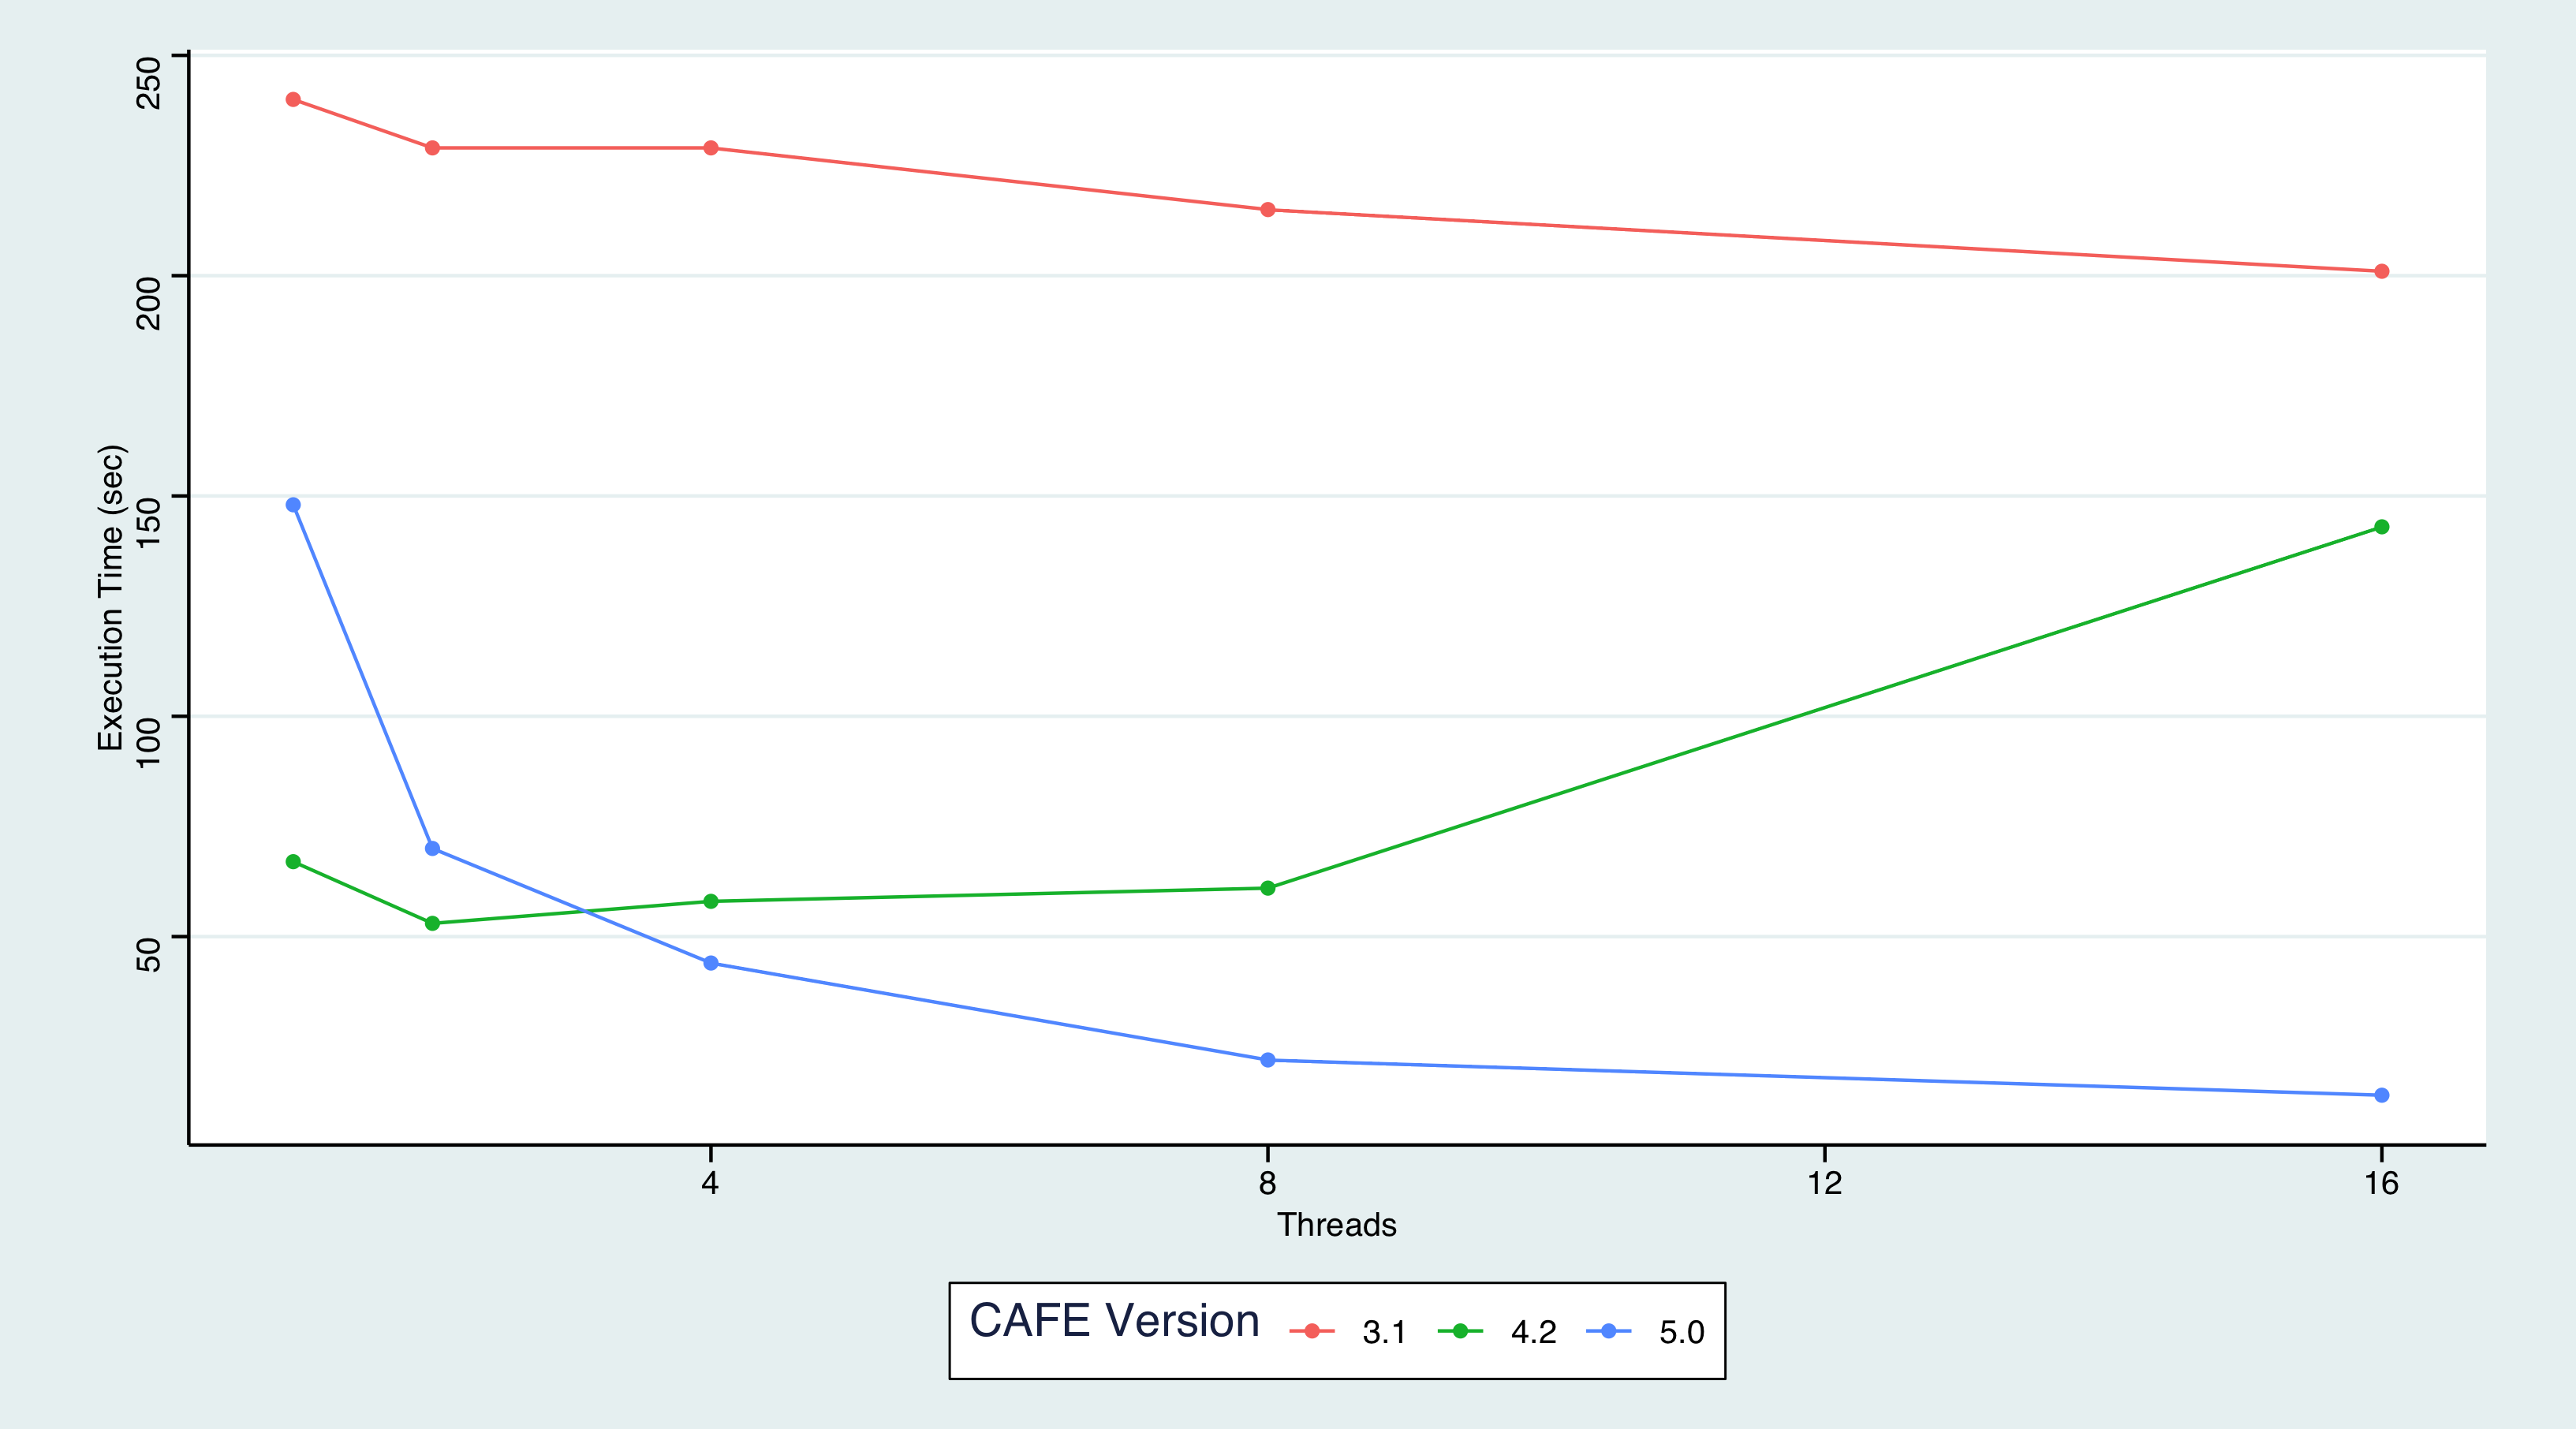
\includegraphics[scale = 0.075]{VersionsThreads}
\caption{Execution times vs. Thread counts for various versions of CAFE using a tree with 10,000 gene families.}
\end{figure}

\subsection{Rewrite}
A new feature for the next release of CAFE had been assigned to a doctoral student. With minimal software engineering experience, the student felt he would be more comfortable creating his own version of the feature rather than attempting to modify the existing code base. After a discussion of the various merits of the C and C++ languages, the decision was made to rewrite the CAFE 4.0 code in an entirely C++ based format. As with any rewrite, this had advantages and disadvantages. With a somewhat clear idea of what the ideal code should look like, it was easier to write the new code in a way that was understandable; still, the CAFE 4 codebase had years of experience and accuracy built into it. 
    
C++ is a more succinct language than C; we were able to replace hash table and linked list implementations from CAFE 4 with language built-ins in CAFE 5. The C++ object-oriented structure allowed us to replace complex code with domain-specific objects that we hoped would be clearer to domain scientists; implementations of Gene Family and Clade classes made clear the primary building blocks of the application. Additionally, the basic similarities between the languages made the transition easier; if we had tried to rewrite the application into Go or Chapel the difficulties might have been much greater.
    
Finding reasons to support a rewrite is simple; much murkier is the task of arguing against it. Code that has been in use for many years often has areas that seem illogical on their face; yet exist to fix some edge-case or odd situation that arose at one point, and this information can be lost in a rewrite. Optimizations that may have been performed on an ad-hoc basis may get lost in the shuffle. As one can see in figure \ref{fig:versionscale} and table \ref{tab:versionscale}, the single-threaded performance of CAFE 5.0 is significantly worse than the previous version; we suspect some subtle modification designed to tune performance may have been missed.

The decision was made to simultaneously work on the rewrite and introduce a major new feature: Allowing lambda values to vary along a gamma curve. Classes were introduced to model the original CAFE lambda model and the new gamma model, and at each step, the output of CAFE 4.2 was carefully tested against the output of CAFE 5.0 to verify no anomalies had been introduced. At the same time, unit tests were added to verify the correct performance of the code. Occasionally, descriptive tests were added to the CAFE 4.2 test base to verify that the results were the same.
    
\section{Results of Performance Optimization} \label{sec:results}

\ben{Optimization: Profile existing code, determine hot-spots (don't miss the forest for the trees), make faster, lather, rinse, repeat..}
    
\ben{Say something about methodology, optimization vs. parallization; hand coding vs. libraries; how good is good enough? (i.e. you need a performance target)}

% \begin{table}[t] \label{tab:familycale}
% \begin{tabular}{@{} *2l @{}}    \toprule
% \emph{Gene Families} & \emph{Execution Time} \\\midrule
% 5000 & 21  \\
%   10000 & 37  \\
%   15000 & 56  \\
%   20000 & 75   \\
%   25000 & 72 \\
%   30000 & 104\\ \bottomrule
%  \hline
% \end{tabular}
% \caption{Execution times of CAFE for various numbers of gene families using CAFE 5.0.}
% \end{table}

\begin{figure}[t] \label{fig:familyscale}
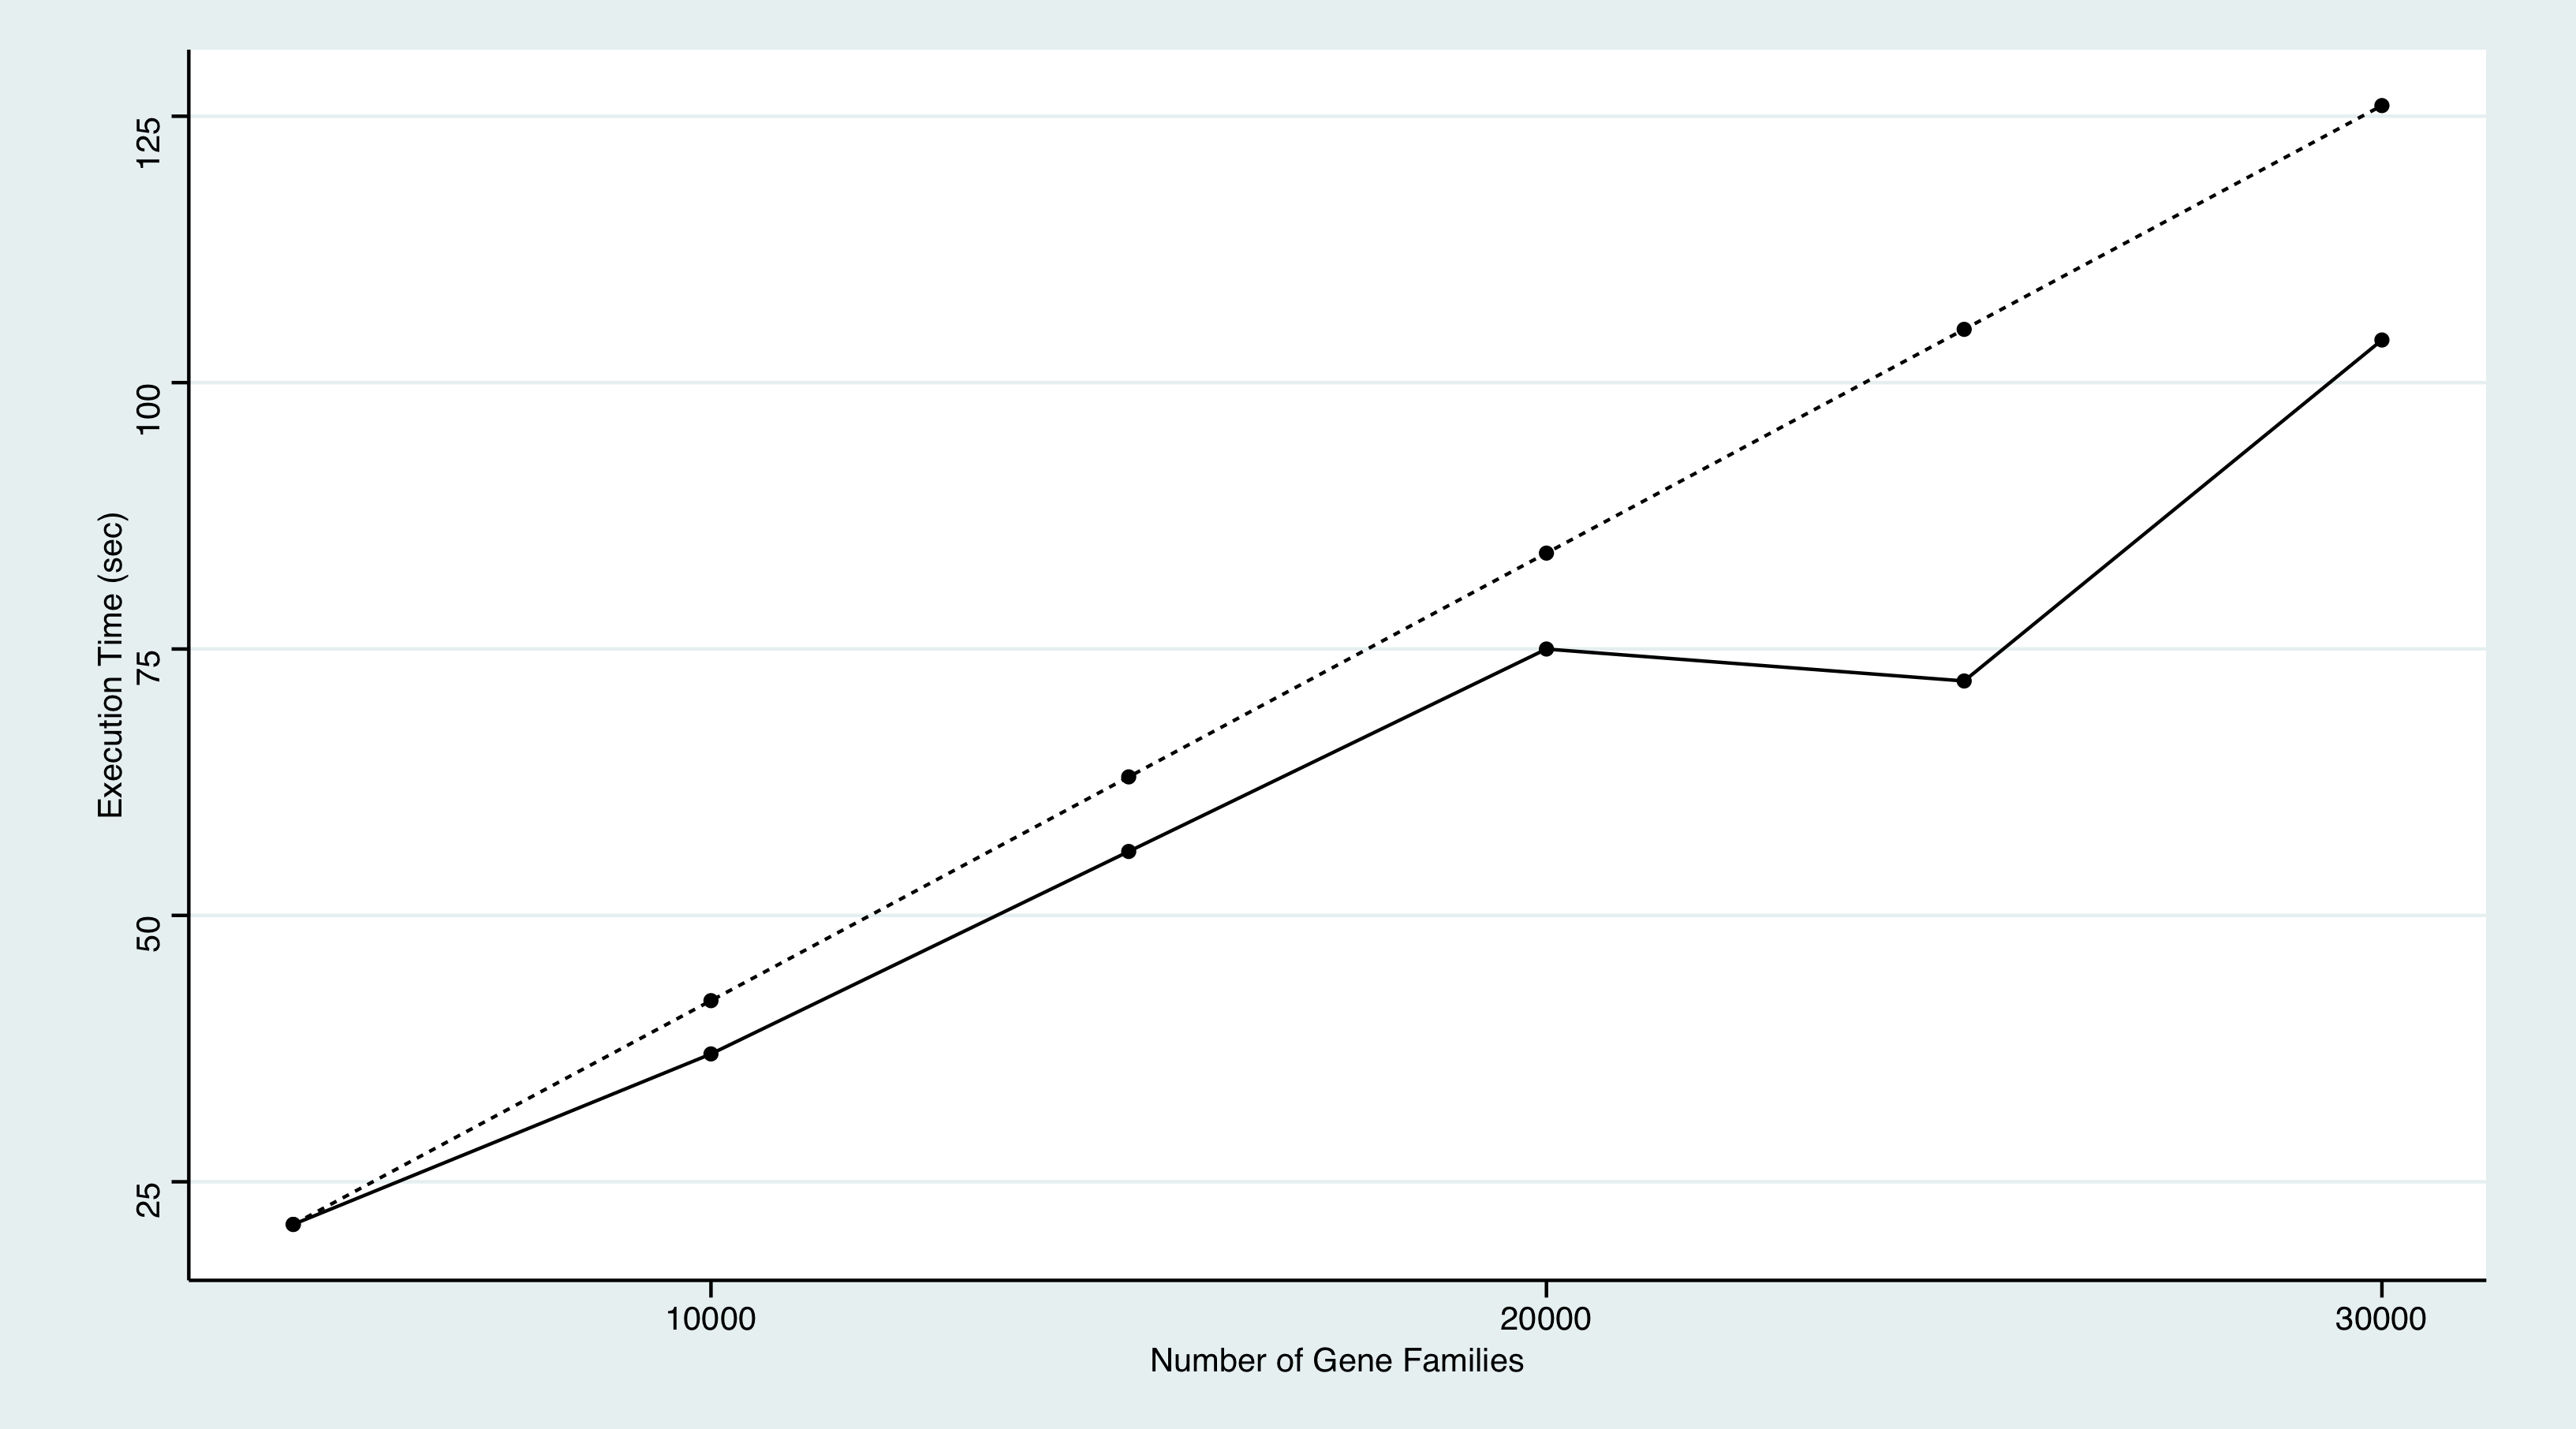
\includegraphics[scale = 0.075]{GeneFamilies}
\caption{Execution times vs. number of gene families for CAFE 5.0 scaling with gene families is nearly linear as indicated by the dashed line.}
\end{figure}

Version 3.1 of the software made some attempts at performance enhancement, via the use of pthreads and some caching mechanisms. In version 4.0, we made some attempts at analyzing the software performance using the Allinea/ARM MAP profiler \ben{expand discussion of tools: profilers, tracers, etc.}, and were able to identify some areas of optimization. Figure \ref{fig:versionscale} and table \ref{tab:versionscale} show the execution times of CAFE for a fixed tree size of 10,000 gene families. One can see that the switch from pthreads in the CAFE 3 series to OpenMP in the CAFE 4 series had a large effect on performance, particularly for smaller core counts. In addition, the OpenMP implementation allowed the code to become cleaner and more relevant to the domain, rather than focusing on the threading model. As the number of threads increased at this problem size, the scaling became worse. In fact, in CAFE 4, although the overall run time is much reduced, the scaling goes in the wrong direction starting with 4 threads. Alternate parallelization methods were considered, such as GPU acceleration and MPI, but were discarded as requiring too many changes to the code base on top of the changes that were already being made.

The configuration option that preferred the Intel compiler over the GCC compiler was a a significant performance gain for those users that could take advantage of it; and the switch to using matrix multiplication libraries, again for those who could take advantage of them, also was a significant gain.

There are three major factors implicated in the performance of CAFE: (1) the size of the tree; (2) the number of gene families to be analyzed (3) the maximum size of a gene family to be considered. This third point deserves some elucidation: Say that a gene family in a given species has 75 members. We wish to determine the probabilities of the clade's ancestor having various member counts. Certainly we will be interested in the the probability of the ancestor having a size of 76, or 70, or perhaps 85; but should we calculate the probability of the ancestor having 150, or 200 members? This is decision is complicated by having to look at the whole tree; if there is one species with a gene family containing 150 members, it is advisable to calculate the probability of any gene family containing that number. The general rule in CAFE is to calculate probabilities up to the largest species size plus 20\%. This factor has a significant effect on performance as can be seen in figure \ref{fig:familyscale}, which shows a nearly linear increase in runtime with the number of gene families considered.

We analyzed the performance of CAFE at three points: v3.1, the final version before an RSE was brought onto the project; v4.2, the final version developed in C and after some initial performance evaluations and modifications had been introduced; and v5.0, the latest version. As we have already shown in figure \ref{fig:versionscale} the v4.2 release following the addition of an RSE brought improved performance. Performance improvement continued on into v5.0 with the rewrite of the code from C to C++. However, the improvement in this case was in the terms of scalability. The single core performance for 10,000 gene families was actually a bit worse for CAFE v5.0 when compared to v4.2, but by the time 4 threads were being used v5.0 was performing better.

Having a code that scales better also translates to improved performance on larger scale problems. Figure \ref{fig:bigscale} shows the performance difference between v4.2 and v5.0 when considering 30,000 gene families. Here we see that v5.0 performs better than v4.2 even at low core counts and continues to see performance improvement (albeit small) all the way out to 32 cores.

\begin{figure}[t] \label{fig:bigscale}
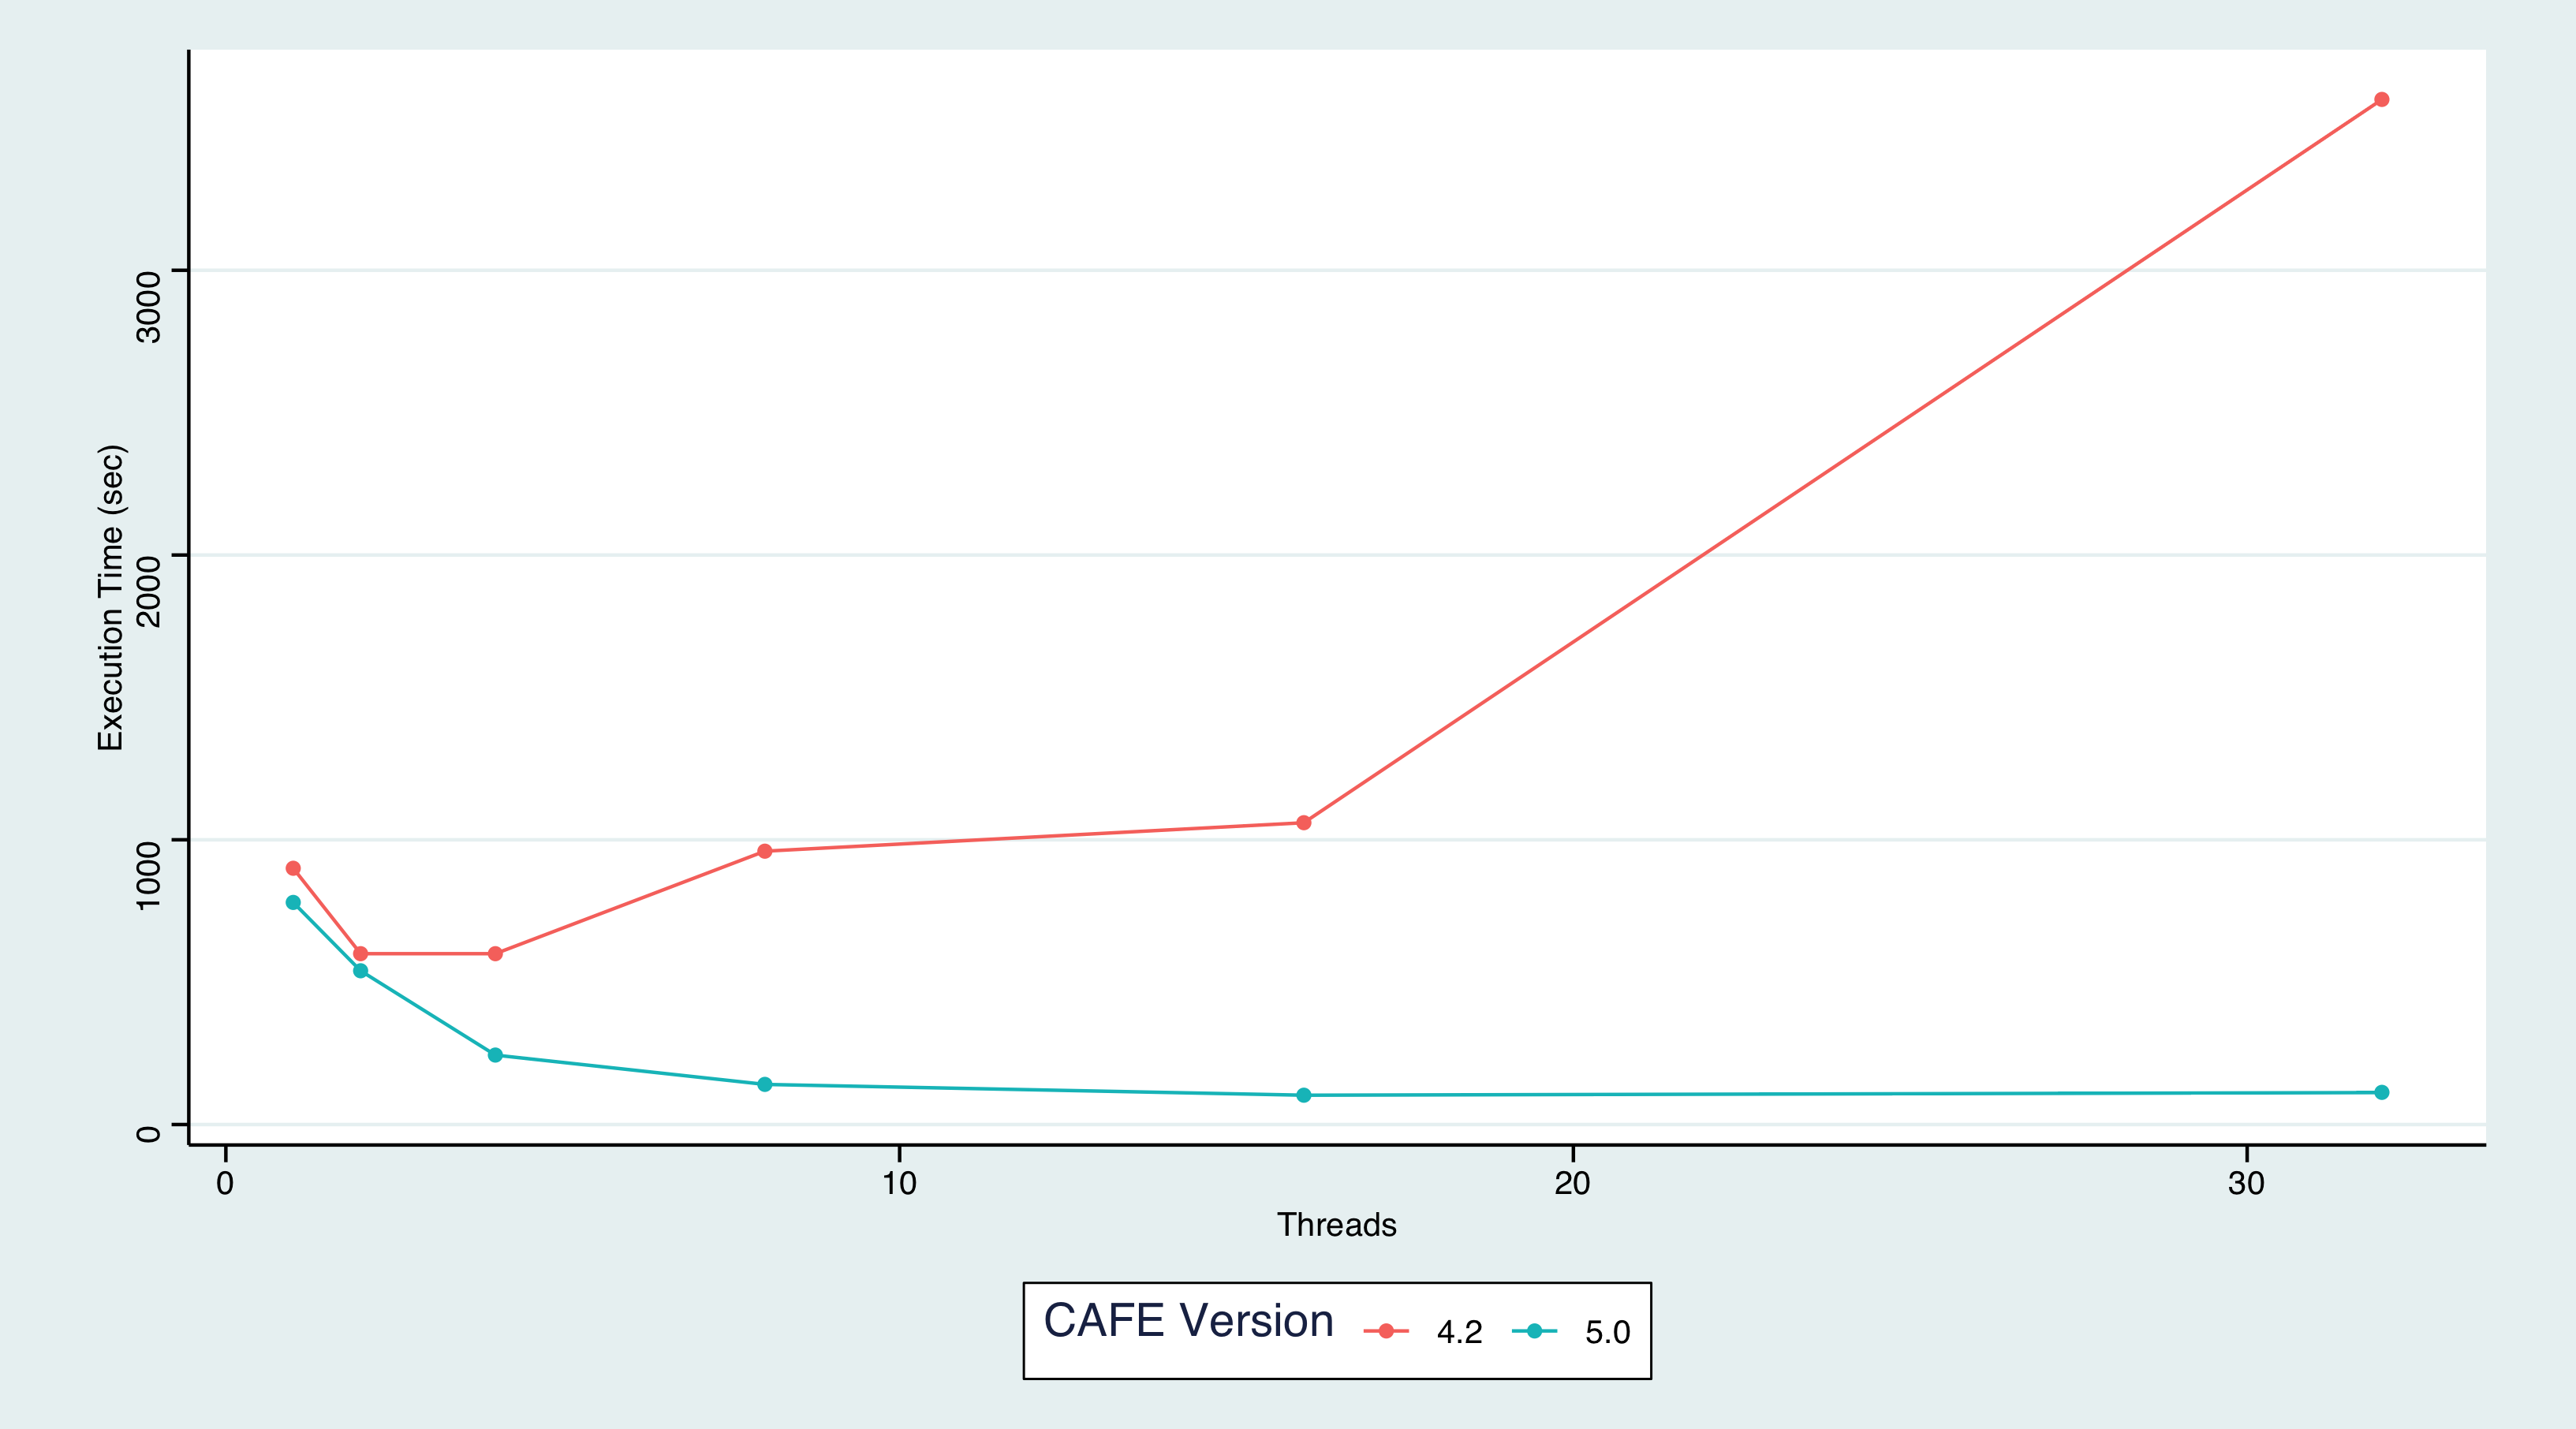
\includegraphics[scale = 0.075]{BigThreadsVersion}
\caption{Execution for CAFE v4.2 and v5.0 for 30,000 gene families.}
\end{figure}

% The performance of CAFE5 as the number of gene families are increased.

% Given a large number (30k) of families to work with, CAFE 5 utilizes 
% available threads effectively.

% \begin{tabular}{ r r r }
%   Threads & v4.2 & v5.0 \\
%   32 & 3600 & 113 \\
%   16 & 1060 & 103 \\
%   8 & 960 & 141 \\
%   4 & 600 & 244    \\
%   2 & 600 & 540    \\
%   1 & 900 & 780
% \end{tabular}

\scott{Look at PEACR facilitation track to find papers to referrence}
  
\section{Discussion} \label{sec:discuss}
Version 5 of the CAFE application is a rewritten version of the application. Written entirely in C++, it is designed to provide a faster and more precise estimation of the lambda value by using a gamma rate to estimate the values. It provides a 2x speedup in the lambda optimization procedure over version 3.1 using a single thread, and a 15x speedup over that version when 16 cores are available. Rather than users creating a script, command-line parameters are used for input values, and various new, user-friendly features are implemented.
    
Online support for the application has been improved greatly via the introduction of a mailing list for users to ask questions. Answers to these questions are provided by both RSE's and domain experts, each providing expertise from their own area. Providing answers to questions has resulted in a "snowball" effect, such that more users are willing to ask questions with the expectation of receiving an answer. In turn, this has facilitated the improvement of the application; for example; v4.2.1 of the software was released when a user reported finding a subtle memory leak.

A consistent challenge that we see at the university is how to provide funding for RSEs to work on software development projects for individual teams and labs. Many faculty have grants that can fund at most a few graduate students or postdoc, but do not necessarily have the budget to employ a full time experienced software developer. Additionally, many projects may not need a full time RSE, particularly if they are only focusing on specific improvements in process or performance. At Indiana University we have used a model of funding several HPC and applications specialists through base university funds, while making some of those individuals time available for work on grants to help improve the development process or performance for scientific codes. This resource has been well received and widely used by faculty throughout the university. Of particular interest is the ability to only pay for a portion of someone's time. In the case of the CAFE grant it was nominally 0.5 FTE, but could vary throughout the course of the grant as needed for new development.
    
    \ben{We were going to say something about Funding for RSE and having happy researchers here}
    
    \ben{Bad things? No handover plan? Mat sabbatical? Rewrite was a bad idea? }

\section{Conclusion} \label{sec:conclude}

Although the general consensus is that revising is better than rewriting for complex software, in this care rewriting worked out well. The code base is easier and cleaner to work with and future coders should have less trouble fixing bugs and implementing new features.

Working in academic research presents a unique set of challenges and opportunities. Although research software design and development tends not to be as rigorously engineered as enterprise software, applying basic software engineering principles to the development of research software can greatly improve the development process and the final product.
% Working in the culture of researchers/professors. pointing out some of the challenges, but also different strengths and opportunities for synergy

%%
%% The acknowledgments section is defined using the "acks" environment
%% (and NOT an unnumbered section). This ensures the proper
%% identification of the section in the article metadata, and the
%% consistent spelling of the heading.
\begin{acks}

This material is based in part upon work supported by National Science Foundation Grant DBI-1564611, and in part by Lilly Endowment, Inc., through its support for the Indiana University Pervasive Technology Institute \cite{stewart2017indiana}. The authors acknowledge the Indiana University Pervasive Technology Institute for providing HPC resources that have contributed to the research results reported within this paper.
\end{acks}

%%
%% The next two lines define the bibliography style to be used, and
%% the bibliography file.
\bibliographystyle{ACM-Reference-Format}
\bibliography{RSEPEARC20}

%%
%% If your work has an appendix, this is the place to put it.
\appendix


\end{document}
\endinput
%%
%% End of file `sample-manuscript.tex'.
